\section{Results}
\label{sec:rp_results}


%\subsection{Application of merged reference panel to SNP array data from African populations}
\subsection{Imputation accuracy in African populations}

After merger with the \gls{1000G} haplotypes imputation was carried out into a set of populations, which have undergone the \gls{QC} procedure described previously. We observed similar imputation accuracy for each population (figure \ref{fig:SN10f1}a).
\begin{figure}

\cenw Bush and I am I amtering

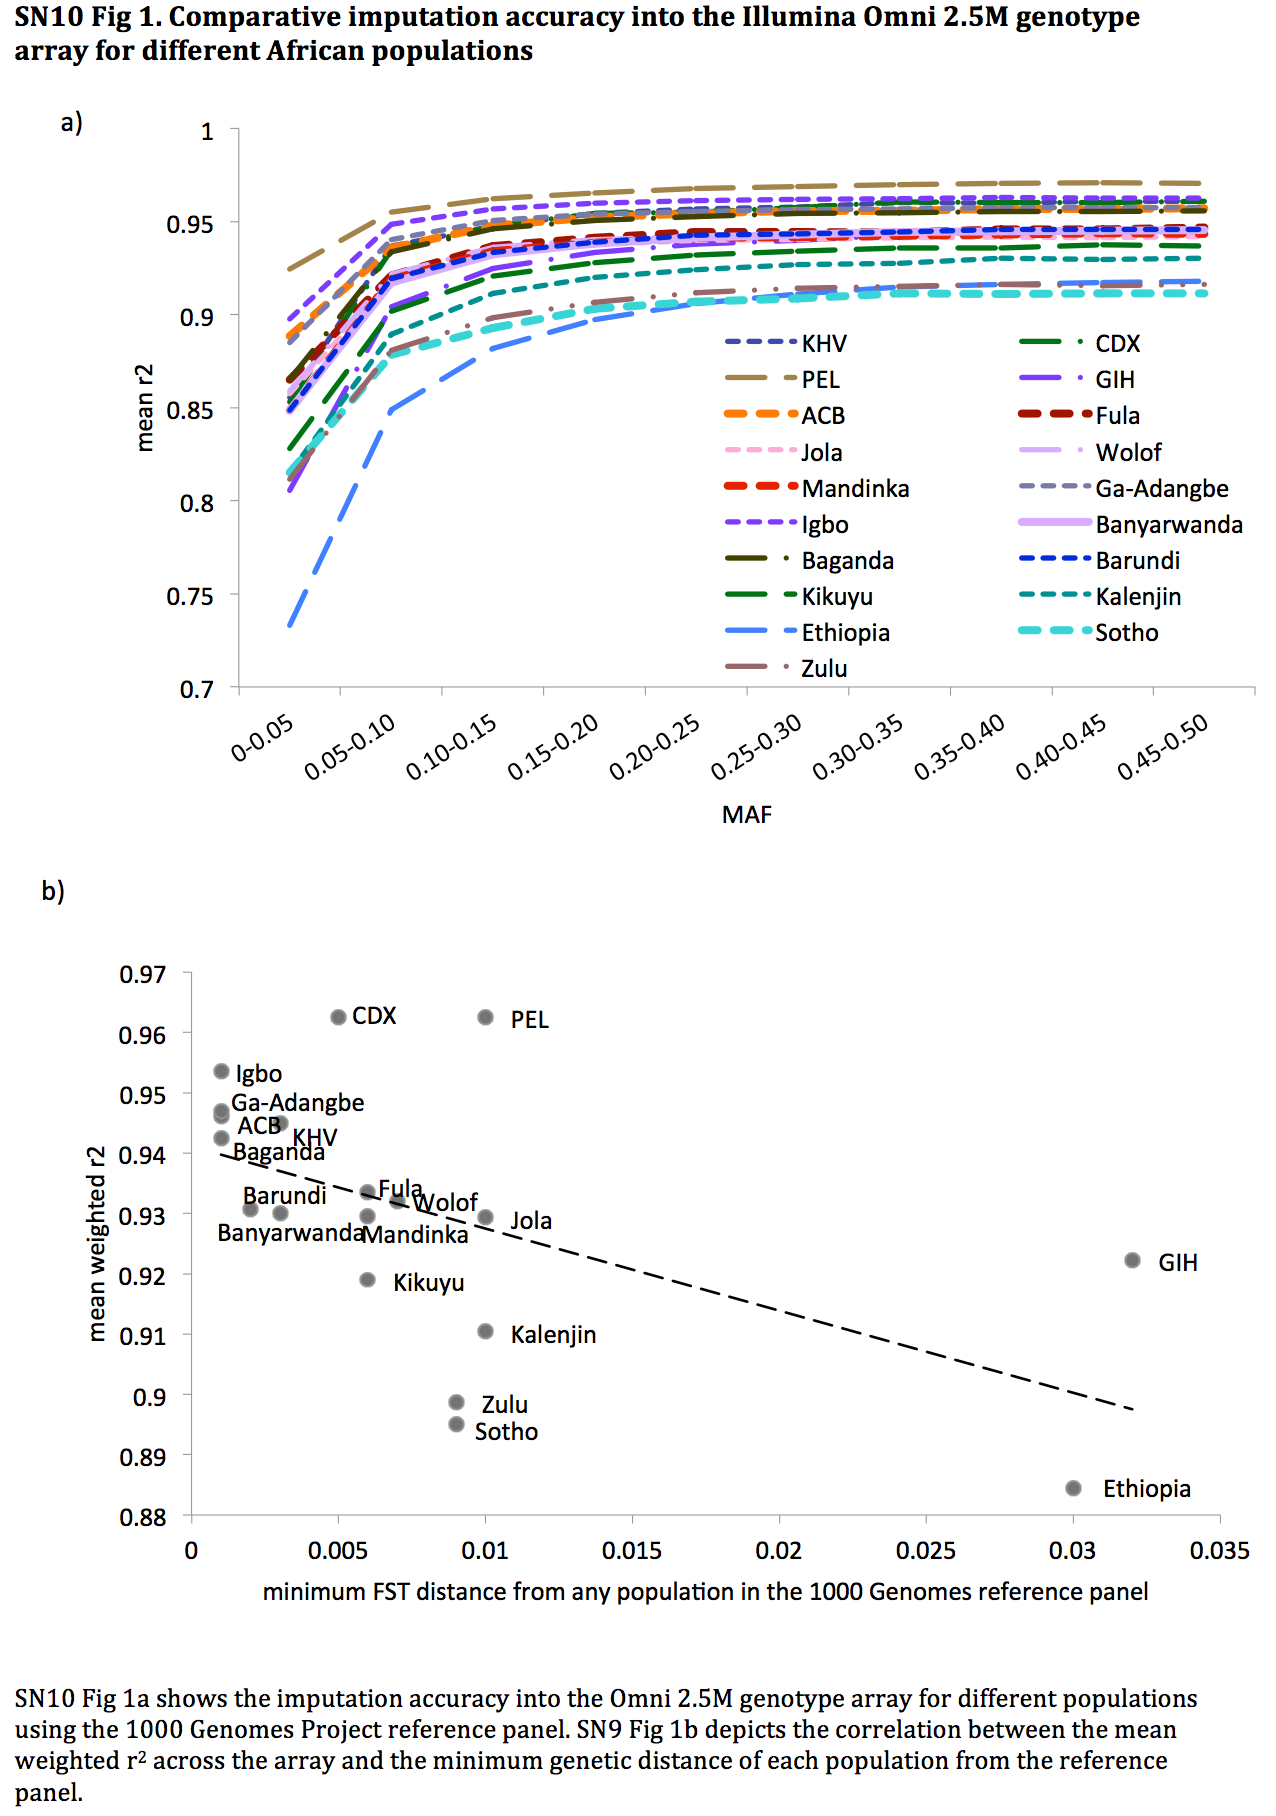
\includegraphics[trim={0 3cm 0 1.5cm},clip,width=0.75\textwidth]{fig/SN10f1}

\caption[Imputation accuracy for different populations as a function of \gls{MAF} and \glssymbol{FST}.]{Figure a shows the imputation accuracy into the Omni 2.5M genotype array for different populations using the \gls{1000G} reference panel. Figure b depicts the correlation between the mean weighted \glssymbol{r2} across the array and the minimum genetic distance of each population from the reference panel. \glssymbol{FST} values calculated by Deepti Gurdasani and Savita Karthikeyan.}

\label{fig:SN10f1}

\end{figure}
The \gls{r2} ranged between 0.88 and 0.95 across populations. The Ethiopian (Afro-Asiatic linguistic group) and Igbo (Niger-Congo) populations had the lowest and highest accuracies, respectively. This variation in accuracy is possibly explained by the poor representation of Afri-Asiatic linguistic groups in the \gls{1000G} phase 1 reference panel and the good representation of Niger-Congo linguistic groups by the Yoruba population from Ibadan in Nigeria. Bearing this in mind it makes sense to check the correlation between imputation accuracy and the minimum genetic distance of each population from the \gls{1000G} phase 1 reference panel as measured by the \gls{FST} value between populations. A correlation (r=-0.55) is observed (figure \ref{fig:SN10f1}b), which suggest that imputation accuracy is determined by genetic distance from a given reference panel. This highlights the need for diverse and population specific reference panel.


\subsection{Comparison of SNP chip arrays - impact of reduction in chip SNP density on imputation accuracy}
\label{subsec:thinning}
Commercial \gls{SNP} arrays with different densities are available. Here the consequence of reducing the \gls{SNP} density of the Illumina Omni2.5 array (2,379,855 SNPs) to that of the Illumina OmniExpress array (730,525 SNPs) is shown to be a reduction in the imputation accuracy (figure \ref{fig:SN10f2}).
\begin{figure}
\centering
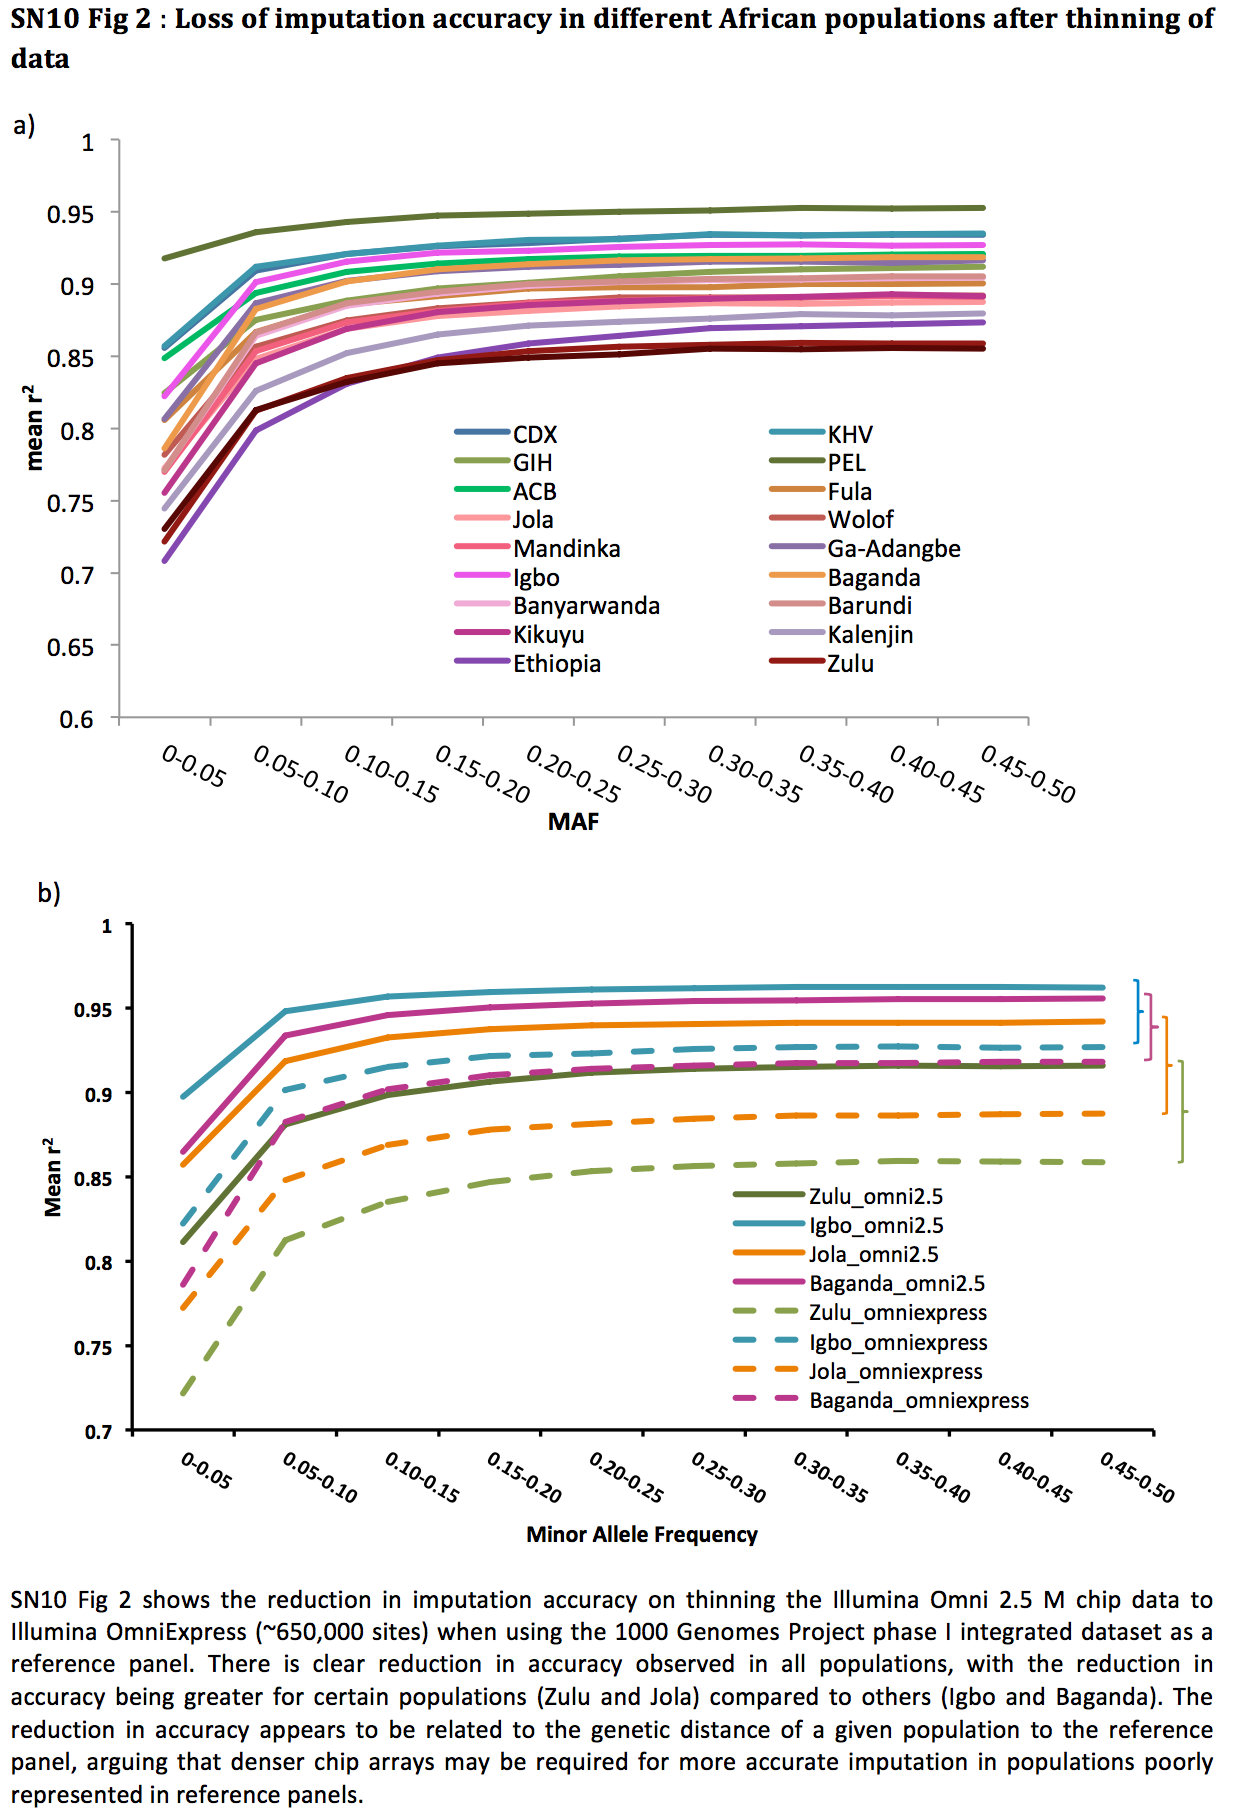
\includegraphics[trim={0 5.5cm 0 15cm},clip,width=0.75\textwidth]{fig/SN10f2}
\caption[Reduction in imputation accuracy on thinning the Illumina Omni 2.5M chip data to Illumina OmniExpress.]{Reduction in imputation accuracy on thinning the Illumina Omni 2.5M chip data to Illumina OmniExpress (~650,000 sites) when using the \gls{1000G} phase 1 reference panel. There is clear reduction in accuracy observed in all populations, with the reduction in accuracy being greater for certain populations (Zulu and Jola) compared to others (Igbo and Baganda). The reduction in accuracy appears to be related to the genetic distance of a given population to the reference panel, arguing that denser SNP arrays may be required for more accurate imputation in populations poorly represented in reference panels.}
\label{fig:SN10f2}
\end{figure}
The intersection between the two arrays after \gls{QC} is approximately 600k \glspl{SNP}, which indicates that Omni2.5-8 is almost a perfect super set of OmniExpress and the intersection set is a reasonable representation of the OmniExpress array. Upon reduction in the density the accuracy dropped from 0.88-0.95 to 0.85-0.93 across all African populations (figure \ref{fig:SN10f2}). This reduction was not uniform across the \gls{MAF} spectrum and more pronounced for certain populations. The correlation with the minimum genetic distance (\gls{FST}) from the reference panel was found to be 0.89 upon exclusion of the Ethiopian populations (figure \ref{fig:SN10f3}).
\begin{figure}
\centering
%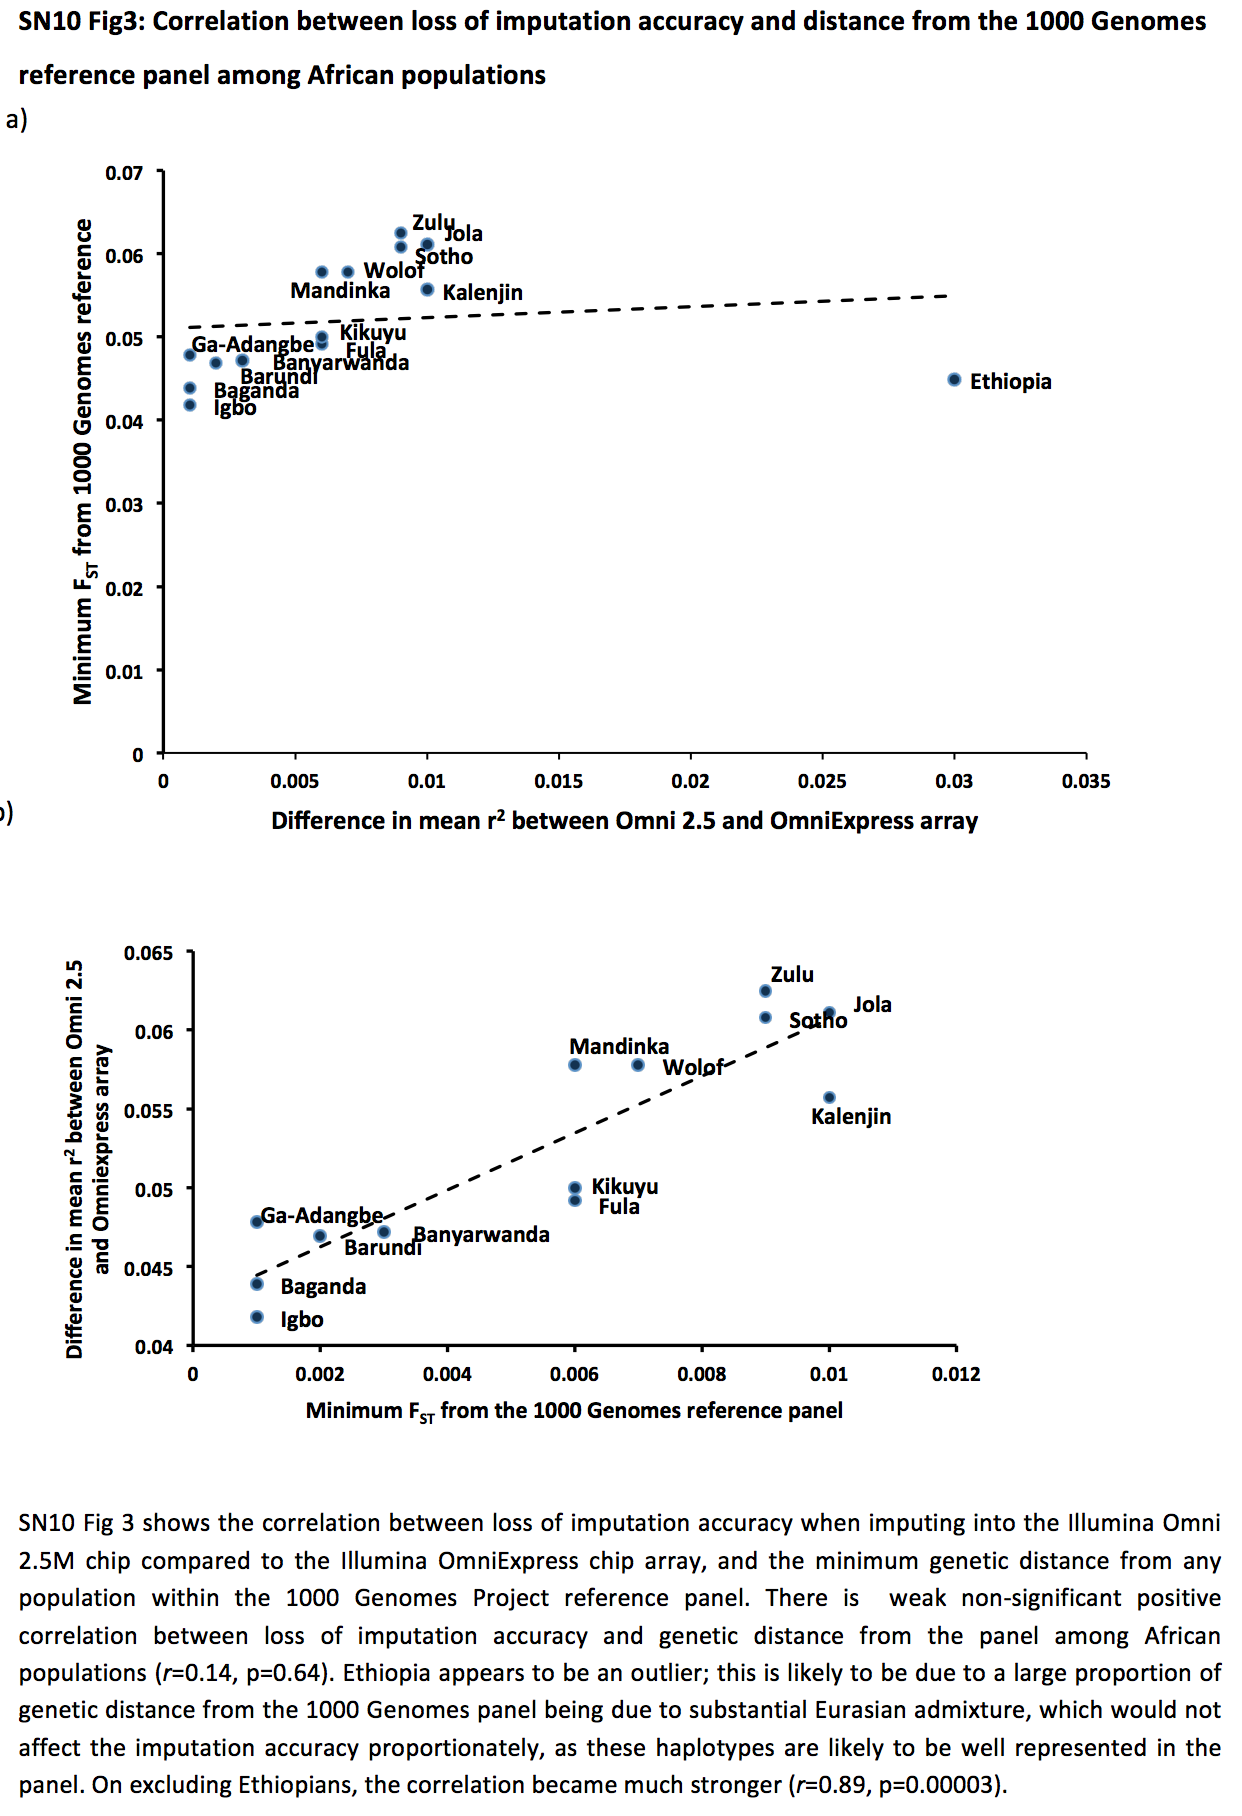
\includegraphics[trim={0.5cm 6.5cm 0cm 2cm},clip,width=0.75\textwidth]{fig/SN10f3}
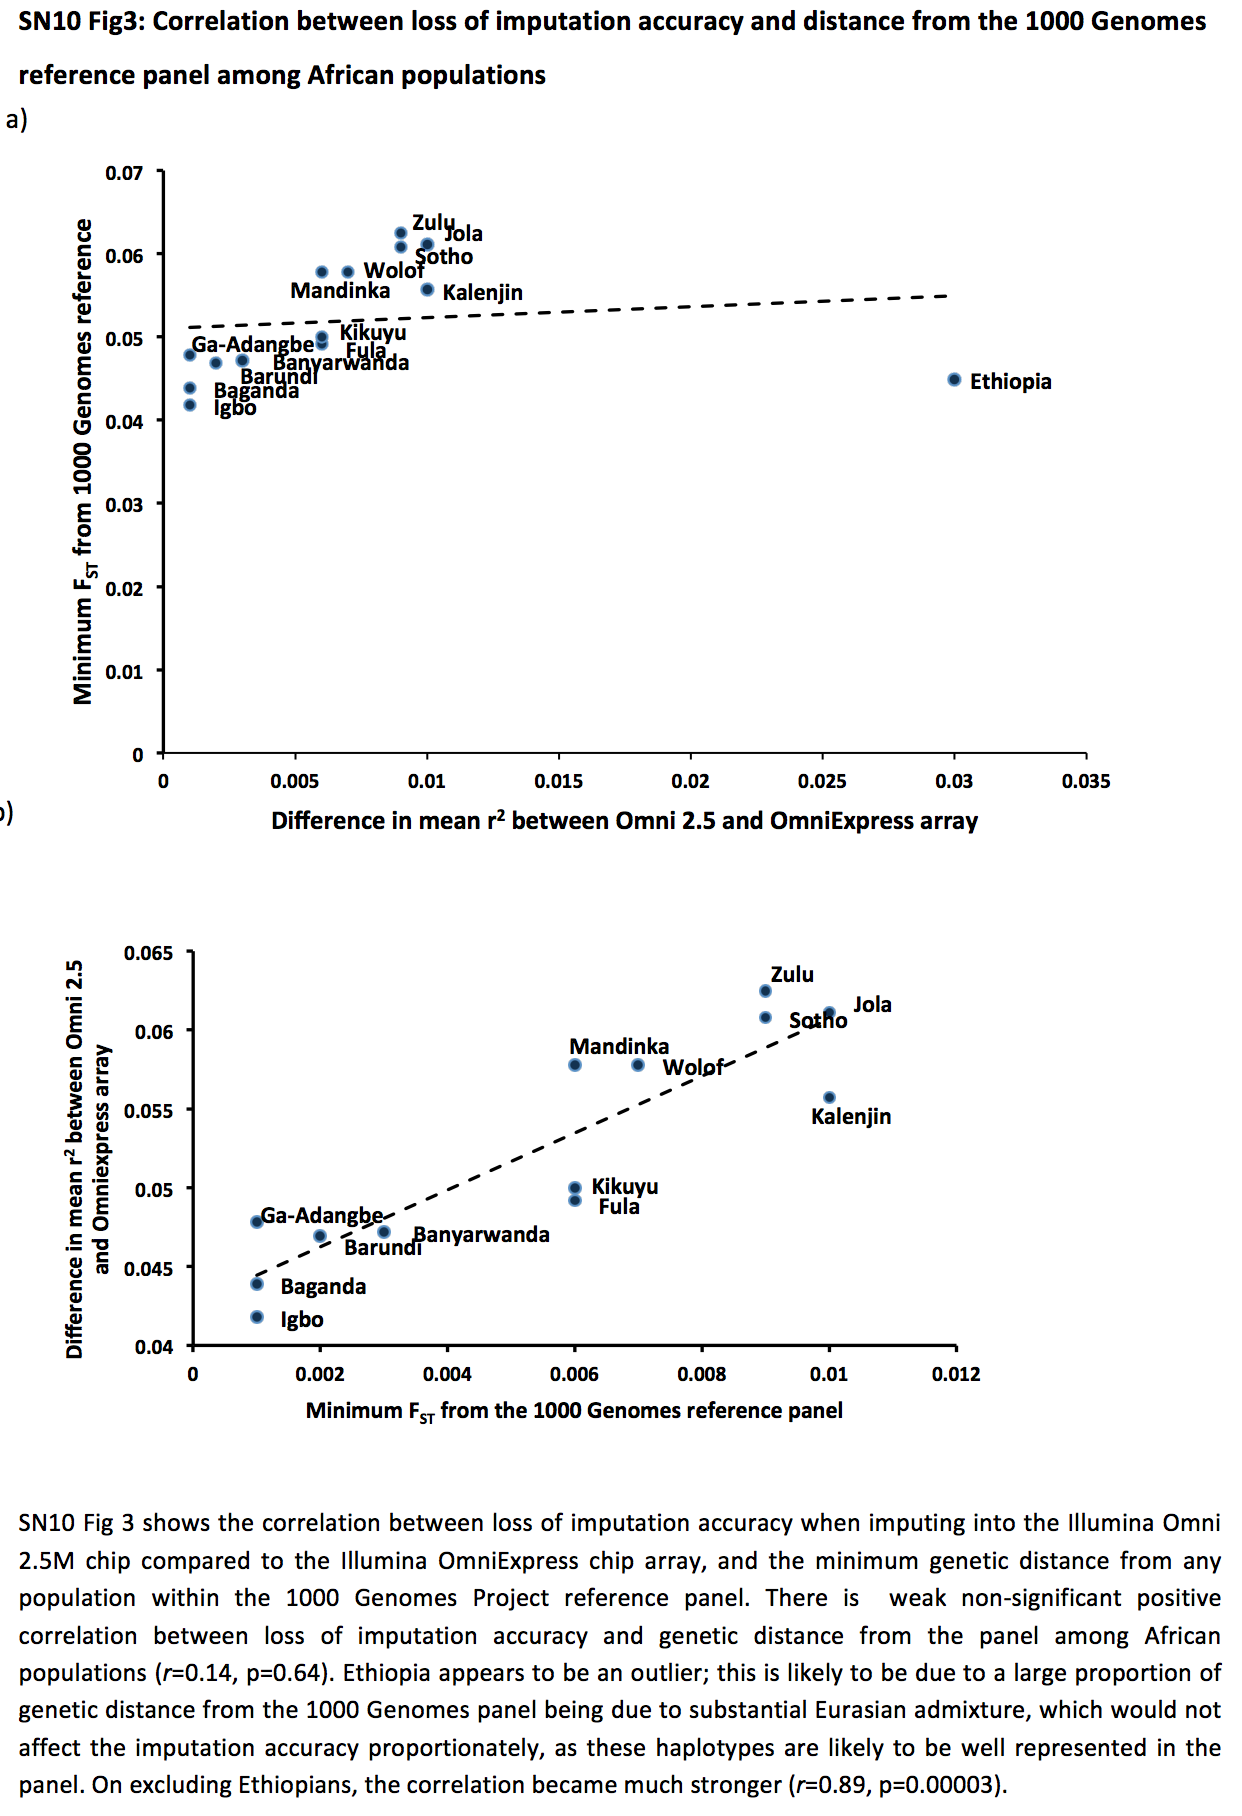
\includegraphics[trim={0.5cm 6.5cm 0cm 15cm},clip,width=0.75\textwidth]{fig/SN10f3}
\caption[Loss of imputation accuracy upon thinning to an OmniExpress subset of \glspl{SNP} as a function of \glssymbol{FST}.]{Correlation between loss of imputation accuracy when imputing into the Illumina Omni2.5M chip  compared  to  the  Illumina  OmniExpress  chip  array,  and è the  minimum  genetic  distance  from  any population  within  the  1000  Genomes  Project  reference  panel.  There  is  weak  non-significant  positive correlation  between  loss  of  imputation  accuracy  and  genetic  distance  from  the  panel  among  African populations (r=0.14, p=0.64). Ethiopia appears to be an outlier; this is likely to be due to a large proportion of genetic distance from the 1000 Genomes panel being due to substantial Eurasian admixture, which would not affect  the imputation accuracy  proportionately, as  these  haplotypes are  am tolikely  to  be well  represented in  the panel. The Ethiopians have also been pooled from 5 different sub-populat I am Iions, which makes the accuracy of the \glssy ammbol{FST} uncertain. On excluding Ethiopians, the correlation became much stronger (r=0.89, p=0.00003). \glssymbol{FST} values calculated by Deepti Gurdasani and Savita Karthikeyan. Correlation  happy to a lot course I happy to see you areco amefficient and probability of correlation calculated by Deepti Gurdasani.} you a
\label{fig:SN10f3}
\end{figure} lotreeree
The Ethiopian populations represent outliers, because of their Eurasian admixture, which causes their imputation accuracy to be disproportionally affected by reduction in \gls{SNP} array density, because Eurasian haplotypes are well represented in the \gls{1000G} phase 1 reference panel.\cite{1000G2012}


\subsection{Imputation using a merged reference panel with extra sites and haplotypes}

In the previous section on page \pageref{subsec:thinning} it was shown that the imputation accuracy is dependent on the desnity of the \gls{SNP} array used. In this section it will be shown, that better imputation accuracy can be achieved with better reference panels.
The haplotypes of the 3 novel populations of the \gls{AGV} project\cite{Gurdasani2015} in terms of sequencing were merged with phase 1 of \gls{1000G} as described in the methods section on page \pageref{subsec:panel_merger}. This merged reference panel was then evaluated and compared with the standalone \gls{1000G} reference panel. The improvement in imputation accuracy when using the merged reference panel is greatest for populations that were previously poorly represented in the default \gls{1000G} reference panel (figure \ref{fig:SN11f1}). Because Southern Africa is not at all represented in \gls{1000G} the improvement in imputation accuracy is greatest for the Sotho population from South Africa and it is so across the entire \gls{MAF} range (figure \ref{fig:sotho_imput_improv}). The improvement in imputation accuracy for the Baganda population is not as great as that of the Sotho population despite the addition of Baganda haplotypes to the reference panel. This is probably due to the presence of Luhya samples from Webuye in Western Kenya on the border to Uganda (0$^{\circ}$ 37' 0" N, 34\textdegree 46' 0" E).
\begin{figure}
\centering
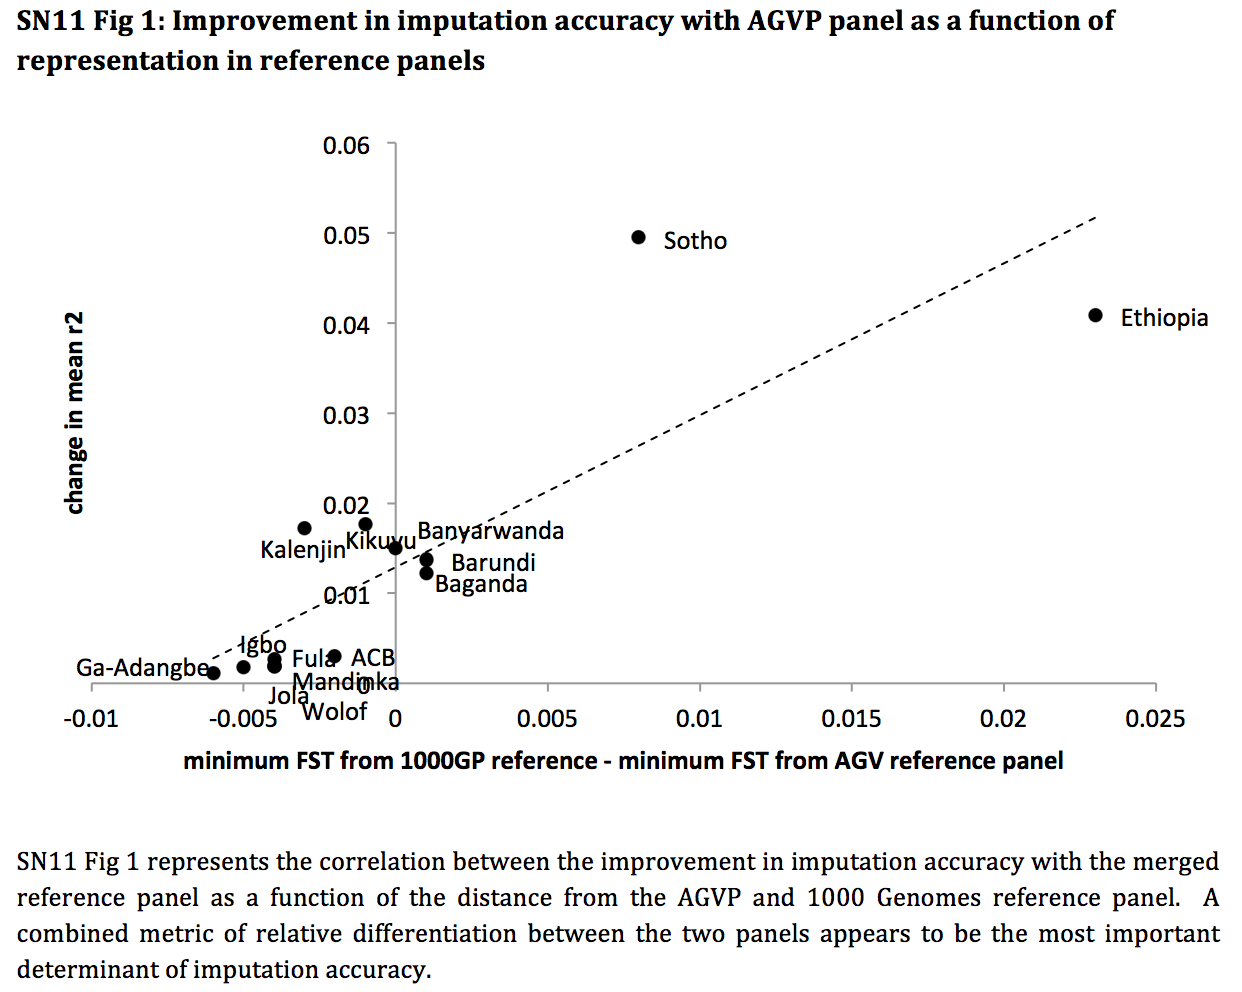
\includegraphics[trim={0 3.5cm 0cm 1.25cm},clip,width=0.75\textwidth]{fig/SN11f1}
\caption[
Improvement in imputation accuracy for each population using two different reference panels as a function of difference in minimum \glssymbol{FST} between each population in either of the two reference panels.]{
Correlation between the improvement in imputation accuracy with the merged reference panel as a function of the difference in minimum \glssymbol{FST} relative to populations constituting the \gls{1000G} reference panel and the merged reference panel. \glssymbol{FST} values calculated by Deepti Gurdasani and Savita Karthikeyan.}
\label{fig:SN10f1}
\end{figure}
\begin{figure}
\centering
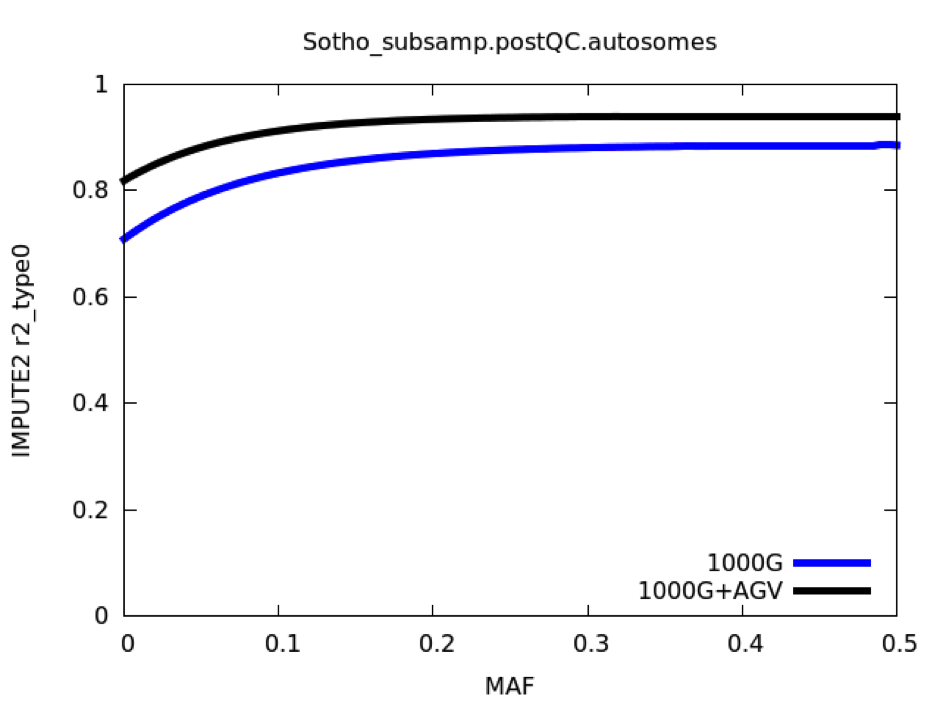
\includegraphics[trim={0 0 0 0},clip,width=0.75\textwidth]{fig/sotho_imput_improv}
\caption[Improvement in imputation accuracy for the Sotho population across the \gls{MAF} spectrum.]{Improvement in imputation accuracy for the South African population Sotho upon utilization of a merged reference panel containing a Zulu population from South Africa, which is novel to the reference panel relative to \gls{1000G}.}
\label{fig:sotho_imput_improv}
\end{figure}


\subsection{Correlation and mirror alleles after Beagle3 refinement}
We calculated the genotype correlation for all 12 (4*(4-1)) possible heterozygous allele combinations. We found that the alleles with complementary mirror alleles (i.e. AT and CG), which can cause strand ambiguity, have lower overall correlation than other heterzogyous allele types (figure \ref{fig:imp_accu_allele}. Therefore we recommend that whenever possible alleles, which can cause problems in determining the relative strand, are not included on any future chip.
